\documentclass{article}
\usepackage{a4wide}
\usepackage{todonotes}
\usepackage[utf8]{inputenc}
\usepackage[T1]{fontenc}
\usepackage{amsmath}
\usepackage{graphicx}
% \usepackage{subfigure}

\title{Response to the Reviewer's Comments}
\begin{document}

\maketitle

We thank the reviewers for their insightful and useful feedback. We have revised our paper in light of their comments. Please, find below our replies and comments about each of the issues raised, and how we modified the paper to address them. Beyond the suggested reviews, we also changes some parts of the paper to adhere to the suggestions. To make clear where we modified, all changes in the text are in blue in this revised version.

\begin{verbatim}
>> REVIEWER #1 <<

> The proposed work simulates underwater imaging sonar based on OpenGL shading
> language (GLSL) chain, and is able to simulate two main types of sonar sensors:
> mechanical scanning imaging sonars (MSIS) and forward-looking sonars (FLS).
>
> The paper is well written with just small issues like "there is any previous
> work for comparison", "foward-looking sonars" or "the sonar simulator can be
> by feature" that needs to be easily solved.
\end{verbatim}

% \todo[inline, color=red!40]{Rômulo's answer}
\textbf{All corrected. Not only the cited typos, but also other
mistakes off the same kind in the revised version. Indeed, we carefully revised the whole text.}

\begin{verbatim}
> The contribution of the work is interesting for the community, mainly if the 
> simulator will become freely available. It can increase the potential of the
> work in terms of impact.
\end{verbatim}

%\todo[inline, color=green!40]{Jan's answer}
\textbf{Certainly, on the acceptance of the paper, we will make the simulator publicly available.}

\begin{verbatim}
> About the work, Figure 3 is confused and needs to be improved. The authors
> argue that the beam are composed by the intensity, depth and angular
> distortion matrix, however it is not clean in the figure. The names makes
> the things hard, please "uniform the names", like "Beam Angle in Camera"
> = "Angular Distortion"? "Surface Angle to Camera" = "Intensity"? "Distance
> from Camera" = "Depth" ?
\end{verbatim}

%\todo[inline, color=green!40]{Jan's answer}
\textbf{Done. We corrected the names in the cited figure (now Fig. 4 in the revised paper) to fit to the text.}

\begin{verbatim}
> In Fig. 6, it is not clear the effect of the parameter "p". How does the
> normal (blue channel) is adopted in the calculus of the acoustic intensity?
> It is more readable to show the final simulation instead of the normal
> image vs. depth image (green channel), as in Fig. 5.
\end{verbatim}

% \todo[inline, color=red!40]{Rômulo's answer}
\textbf{To find the final pixel intensity, we multiply its normal angle value by the material reflectance $\rho$. This operation takes place in fragment shader. We rewrote the sentences on subsection 3.2 to make the idea clearer. Also, the Fig. 6 was modified to take this consideration.}

\begin{verbatim}
> About the simulation resolution, the number of bins are dependent of the
> sonar's frequency and the adopted range. The authors know it, as shown in line
> 266, however it could be interesting to define the number of bins in terms of
> these two parameters to make the simulation "more realistic" in terms of
> the real sensor. It could be interesting for the community.
\end{verbatim}

%\todo[inline, color=green!40]{Jan's answer}
%%%Luciano 03/06/2017: não entendi a última parte da resposta; a parte do "driver"!!!!!
\textbf{The simulator itself is as freely parameterizable as possible to allow for a wide range of imaging sonars to be simulated. The definition of the bin numbers, ranges etc. is done for each individual simulated sonar in the corresponding component which injects the sonar data into the full simulation. For example has the driver for a simulated TriTech Gemini sonar for the exact same parameters as the real sonar. From the point of view of the robot control, the system can be very realistic.}

\begin{verbatim}
> Another interesting thing is related to the noise simulation. It does not appear
> realistic due to the lack of "noise" in the black areas. The application of
> noise in this area can be interesting.
\end{verbatim}

% \todo[inline, color=red!40]{Rômulo's answer}
\textbf{This issue is explained in subsection 4.1. As we described in
Section 3.4, the speckle noise modeled in this paper is a multiplicative one,
following a non-uniform distribution. The resulting sonar data is composed by
an element-wise multiplication between the raw data and the speckle noise. The
insertion of additive noise is already addressed as future work to solve this
missing part.}

\begin{verbatim}
> The main limitation of the work is the lacks of reverberation simulation in the
> work. It limits the applicability of the simulation to open waters with a small
> number of objects. Thus, it appears to be the "main future works", however, the
> authors do not mention it.
\end{verbatim}

% \todo[inline, color=red!40]{Rômulo's answer}
%%%Luciano 03/06/2017: O que é "outlook section"?
\textbf{We have chosen to extend the underwater acoustic phenomena in the
simulator obeying the use by real-time applications. Processing the
reverberation in a sonar simulator is computationally costly, then its
addition must consider the time consuming again. We took this problem
into account and addressed it as future work in the outlook section.}

\begin{verbatim}
> It is hard to validate a simulator, however, I believe the works lake in
> terms of comparison with real data at least in terms of SNR or other metrics.
> It could be interesting to simulate a "real scenario" and compare the results
> obtained by the simulator.
\end{verbatim}

%\todo[inline, color=green!40]{Jan's answer}
%%%Luciano 03/06/2017: Tem que revisar esta resposta. Já não condiz com o texto!!!!!
\textbf{We just now had the opportunity to record data with an imaging sonar of an object which we can fully simulate (see Figs. 7(c) in the revised paper and \ref{fig:real_sonar} of this document). Therefore we plan to use this data next months to analyze the quality of the simulation and publish this later when the results are satisfied.}
\newpage

\begin{figure}[tb]
    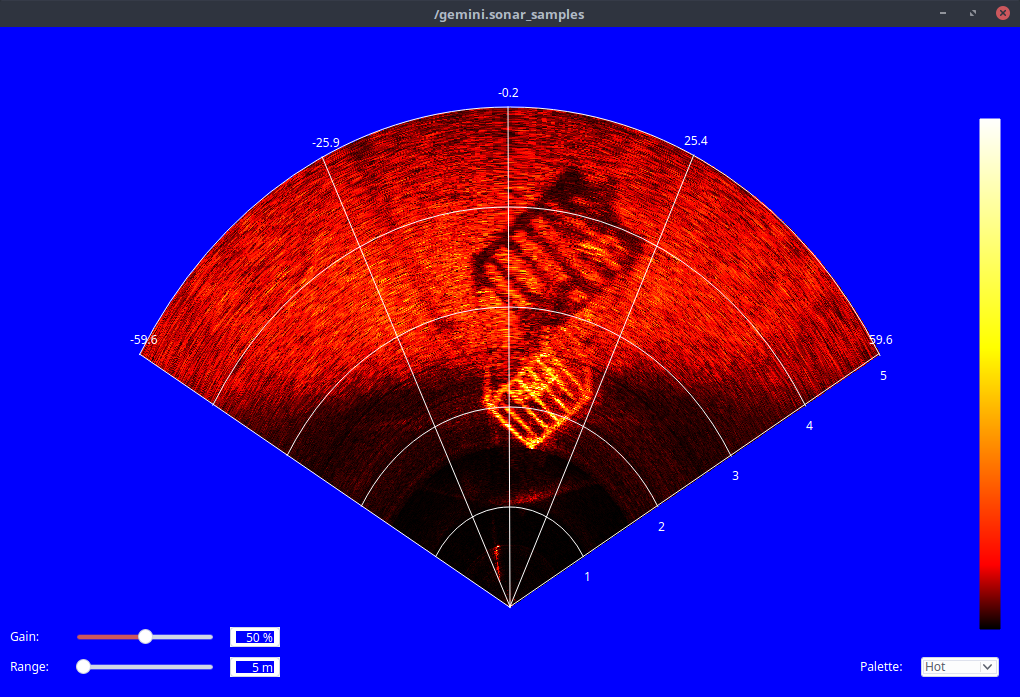
\includegraphics[width=0.7\columnwidth]{figs/real_ssiv}
    \centering
    % \captionsetup{justification=centering}
    \caption{Image of a Tritech Gemini 720i Imaging Sonar of a mock-up of a sub-sea structure.}
    \label{fig:real_sonar}
\end{figure}

\begin{verbatim}
>> REVIEWER #2 <<

> The Euclidean distance from camera center, the surface normal angles, and the
> angular distortion are recorded as color channels. In this case, there is a
> limitation of 256 values. Does this brings precision problems? Using CUDA or
> OpenCL, couldn't this be addressed in a more elegant way?
\end{verbatim}

% \todo[inline, color=red!40]{Rômulo's answer}

\textbf{The only problem caused by the limitation of the 8-bit channel
representation is in the Euclidean distance from camera center information (let us call this information as depth). In this case, we replaced the original depth information by the native GLSL depth buffer, which has 32-bit floating-point values. In fact, this information was not addressed in the first version of the paper. We clarified this issue in the revised version. }

\textbf{Indeed, CUDA and OpenCL are both good alternatives to implement
the proposed approach. However, we have chosen to use GLSL for three main reasons:
1) native from OpenGL, avoiding to install additional packages;
2) hardware and backward compatibility;
3) use of precomputed geometric information during the rasterization process.}

\begin{verbatim}
> I would like to see more details on the implementations of the models. I am not
> sure if it is possible to reproduce the solution with the presented text.
\end{verbatim}

% \todo[inline, color=blue!40]{Undefined responsible's answer}
\textbf{We added as much details as possible in this revised version. Conditioned to the acceptance of the paper, the simulator will be available under an open source license and may be downloaded from Github.}

\begin{verbatim}
> This sentence seems to be from a decade ago paper…: Modern graphics hardware
> presents programmable tasks…
\end{verbatim}

% \todo[inline, color=red!40]{Rômulo's answer}
\textbf{This sentence was removed in our revised manuscript.}

\begin{verbatim}
> It is unclear to me, but each beam is for a complete column?
\end{verbatim}

% \todo[inline, color=red!40]{Rômulo's answer}
\textbf{Each beam is composed by one or more columns, according to sonar
bearings. We took this point into consideration, rewriting the text to make
it clearer.}

\begin{verbatim}
>> REVIEWER #3 <<

> The present work proposes a method for the simulation of sonar sensors.
> Differently from previous methods, the proposed technique takes advantage
> of the GPU to achieve realtime performance and is able to reproduce the
> operation of FLS and MSIS sonars sensors.
>
> Text
> ====
>
> The text contains some confusing passages that demand review. For instance:
>
> --- lines 78-82
> "The intensity measured back from the in-
> sonified objects depends on the accumulated energy based on
> surface normal directions, producing more realistic simulated
> scenes, instead of statically defined by the user, as in [5], or in
> a binary representation as found in [6, 7]."
>
> ---> "accumulated energy" refers to what exactly? Energy accumulated where?
> ---> "instead of statically defined by the user" What does it mean?
\end{verbatim}

% \todo[inline, color=red!40]{Rômulo's answer}
%%%Luciano 03/06/2017: rever se está realmente claro essa questão do energy accumulated. Acho que não, ainda.
\textbf{We rewrote this paragraph to clarify these issues.}

\begin{verbatim}
> --- lines 172-174
> "The Rock-Gazebo integration [17] provides the underwa-
> ter scenario, and allows real-time hardware-in-the-loop simula-
> tions."

> ---> What is "Rock-Gazebo integration"? The authors explain it later. However,
> the order of the sentences could be switched to make text a bit clearer.
\end{verbatim}

%\todo[inline, color=green!40]{Jan's answer}
%%%Luciano 03/06/2017: rever a resposta. Mudamos isso depois.
\textbf{This sentence was rewritten in the revised version to explain the necessity of the integration of the sonar simulation into a framework and then the connection to Rock-Gazebo was made. That hopefully makes this paragraph a less confusing.}

\begin{verbatim}
> The Introduction section contains some text that should be in the Related
> Work Section.
\end{verbatim}

%\todo[inline, color=yellow!40]{Luciano's answer}
\textbf{We decided to include the related work continuously inside the introduction without a dedicated subsection. We think that it makes the text more uniform and fluid in the introduction.}

\begin{verbatim}
> Technically, bump maps are different from normal maps. Bump maps are defined as
> height maps that describes the bumps on parametric surfaces. Normal maps, on the
> other hand, are textures that contain perturbed normal vectors. There are both
> tangential and object space normal maps. It seems that the proposed technique
> uses normal maps. I suggest a review on that.
\end{verbatim}

% \todo[inline, color=red!40]{Rômulo's answer}
\textbf{In fact, the proposed approach uses normal maps to simulate geometric surface irregularities by passing RGB textures and modifying the normal vectors. We revised the manuscript to change this.}

\begin{verbatim}
> Some image labels are too small.
\end{verbatim}

% \todo[inline, color=red!40]{Rômulo's answer}
\textbf{The paper have followed the journal's LaTeX template. It is not possible to modify this point.}

\begin{verbatim}
> No need to put "the {first|second|third|last} {scenario|scene}" in bold on
> lines 322, 327, 334, 343, 347-348, 354-355.
\end{verbatim}

\textbf{The rationale in putting the sentences in bold was to highlight the beginning of the explanations about each scene/scenario. This helps the reader to follow our description.}

\begin{verbatim}
> Contributions and limitations
> =============================
>
> In the abstract the authors state the importance of simulating sonar sensors
> and then introduce the proposed method. However, nothing is said
> about the difficulties involved in such a simulation and about the general
> limitations of current methods. Along the text, it seems that the use of the GPU
> for sonar sensor simulation is a contribution, but this is not mentioned in the
> abstract.
\end{verbatim}

\textbf{We added the use of GPU in the abstract. In fact, we completely revised the abstract to fit to the suggested changes.}


\begin{verbatim}
> --- lines 69-73
> "This paper introduces a novel imaging sonar simulator, that
> can overcome the main limitations of the existing approaches.
> As opposed to [1, 2, 3, 4, 5, 6, 7], where the proposed models
> simulate a specific sonar type, our model is able to reproduce
> two kind of sonar devices (...)"
>
> ---> These sentences may lead the reader to wrongly interpret the existing
> techniques, that simulate only one type of sensor, as being limited although
> they could even do it very accurately. Actually, it can be (and probably will
> be) the case that the authors of the existing techniques were not concerned
> about simulating several sonar sensor types. I think that this statements should
> be reviewed and rewritten in order to correctly account for that.
\end{verbatim}

% \todo[inline, color=green!40]{Jan's answer}
\textbf{We have rewritten the sentences and the paragraph to avoid such confusion and make them clearer.}

\begin{verbatim}
> ---> The authors claim that the proposed technique overcomes the "main
> limitations" of existing techniques. However, the proposed method itself
> introduces limitations that were not present in some of the existing techniques
> (for instance, the proposed method does not handle reverberation, an important
> phenomenon in the context of sonar sensor simulation). Thus, I think that the
> discourse about contributions versus limitations should be reviewed in order
> to be fair.
\end{verbatim}

% \todo[inline, color=green!40]{Jan's answer}
\textbf{We addressed your consideration in the text and rewrite the
subsection 1.1 to avoid such confusion in the revised paper.}

\begin{verbatim}
> The method
> ==========
>
> The explanation about sonar sensors, and how they work, seems to be Ok. However,
> I've missed a formalization of the problem being simulated. Without it, it
> becomes difficult to understand how good the proposed simulation method is
> (which were the simplifying assumptions adopted?). Also, the description of
> the method implementation is quite confusing. I think that a grad student
> could not implement it without too much guessing.
\end{verbatim}

%\todo[inline, color=green!40]{Jan's answer}
\textbf{We tried to incorporate all your suggestions and hope to clear out our description of the method.}

\begin{verbatim}
> --- lines 74-78
> "Also, the underwater scene is processed during the pipeline rendering on
> graphics processing unit (GPU), accelerating the simulation process,
> guaranteeing real-time simulation, in contrast to the methods found in
> [1, 2, 4, 5]."
>
> ---> It is not clear why the GPU/rasterization were chosen and how the GPU
> helps in overcoming eventual problems/limitations of the existing techniques.
> Why GPU-based realtime ray tracing was not chosen, for instance?
\end{verbatim}

% \todo[inline, color=blue!40]{Undefined responsible's answer}
\textbf{The rasterization was chosen because the geometric data from virtual
scene are computed on optimized pipeline GPU embedded. With this, we handled with
these precomputed data to get the depth, intensity and angular distortion parameters needed to build the acoustic frame. In addition, we have rewritten the subsection 1.1 to include these informations.}

\begin{verbatim}
> The method takes advantage of the rasterization pipeline in order to build
> the distance, normal and angle maps. This is not stated anywhere, but that
> rendering method is similar to the "deferred shading" (which solves the
> visibility from the camera viewpoint at the same time that stores several
> properties of the rasterized fragments into an auxiliar buffer). This would
> be one advantage related to the use of GPU in this context.
>
> From Section 2 (lines 104-107) it seems that bins are samples placed along the
> beam. However, I could not spot how these samples are obtained from the
> description in Section 3.3. Actually the text explains it, but I've found it too
> confusing. In the beginning I had the impression that the distance, angle and
> normal maps were 2D. Later on, I started thinking that they should be 3D
> (what does "3D shader matrix" mean in line 257?). However, if they are really
> 3D maps, when is each slice of this 3D map (matrix) obtained? I've got really
> confused at this point.
\end{verbatim}

% \todo[inline, color=green!40]{Jan's answer}
\textbf{The "3D shader matrix" is a 3-channel matrix which stores the information about depth, intensity and angular distortion from the captured OSG scene. We have rewritten this term on paper to make it clear.}

\begin{verbatim}
> I've found the noise model too arbitrary. How good is this approximation?
\end{verbatim}

% \todo[inline, color=blue!40]{Undefined responsible's answer}
\textbf{The speckle noise $n$ is a bell curve, following a Gaussian non-uniform
distribution:}

\begin{equation*}
n(x;\mu,\sigma) = \frac{1}{{\sigma \sqrt {2\pi } }}e^{{{ - \left( {x - \mu } \right)^2 } \mathord{\left/ {\vphantom {{ - \left( {x - \mu } \right)^2 } {2\sigma ^2 }}} \right. \kern-\nulldelimiterspace} {2\sigma ^2 }}},
\end{equation*}

\textbf{given mean $\mu$ and standard deviation $\sigma$. In the proposed approach, we defined $\mu = 0.4$ and $\sigma = 0.15$, and the modeled curve is presented in Fig. 4(v) in the paper.}

\begin{verbatim}
> Results
> =======
>
> --- lines 86-88
> "The main goal here is to build quality and low time-con-
> suming acoustic frames, according to underwater sonar image
> formation and operation modes (see Section 2)."
>
> ---> The Results Section does not compare the obtained results with data
> obtained with real sensors (validation). The proposed method is not even
> compared to existing techniques (except for speed in some cases). Thus, despite
> the fact that the proposed method can very efficiently simulate two distinct
> types of sonar sensors, it is not possible to assert how good the results are
> (quality).
\end{verbatim}

%\todo[inline, color=green!40]{Jan's answer}
\textbf{With regards to other simulation systems, we have the problem that the freely available simulators either don't fit our targeted niche of having a real-time simulation for robots or are bound to specific sonar they simulate. This is the one of the reasons we actually started our development. Real sonar data validation is incredible hard, since there are a lot of parameters to consider. We
will however conduct a qualitative comparison using data we were able to record very recently. A paragraph pointing this out has been added to the results section.}

\begin{verbatim}
> --- lines 370-373
> "In real sonar images, the noise also granulates the shadows and blind regions.
> The sonar simulator can be improved by inserting an additive noise to our
> model."
>
> ---> This seems to be a feature that could be easily included. Why it was not
> added to the system?

\end{verbatim}

%\todo[inline, color=green!40]{Jan's answer}
\textbf{Additive noise has a far more sever impact on the image and therefore on any recognition algorithm running on that image. It is therefore very important not to divert too far from the real world, which is why we e.g. haven't just added a Gaussian additive noise. There is ongoing work to integrate it, but we are not finished. We added a short sentence in the test explaining this situation.}

\begin{verbatim}
> Here I make an observation regarding the proposed technique. As was
> mentioned in the paper, several existing techniques make use of the ray tracing
> in order to simulate sonar sensors because reflection is extremely
> important in the context of sound propagation simulation and it
> can be easily simulated with ray tracing. Thus, how do the authors
> plan to efficiently expand their rasterization-based system in order to handle
> reflections? Wouldn't it be easier and more efficient with GPU-accelerated ray
> tracing?
\end{verbatim}

% \todo[inline, color=green!40]{Jan's answer}
\textbf{Good point. We have decided to extend the physical phenomena in the
simulator obeying its usage in real-time conditions. Knowing that, our approach
is optimized by taking precomputed geometric data during the rasterization
pipeline on GPU to compute the acoustic frame instead of simulating sound pulse propagation with ray-tracing approach. Computing the multi-path reflection in sonar simulation is computationally costly, thus we need to consider the time consuming again by modeling and including phenomena such as reverberation. This will be made in the future.}

\begin{verbatim}
> --- lines 373-375
> "This lacking part can be addressed by implementation of a multi-path propaga-
> tion model."
>
> ---> What does it mean "multi-path"? References?
\end{verbatim}

% \todo[inline, color=red!40]{Rômulo's answer}
%%%Luciano 03/06/2017: Isso está bem explicado no texto? Veja ai.
\textbf{Multipath means that a signal propagates between transmitter and receiver along several different paths, resulting in fading and reverberation effects. We included the reference [22] in the paper.}

\begin{verbatim}
> Decision
> ========
>
> The proposed work is very interesting but seems to be just in early stages
> of development. Some decisions were not very well justified (why GPUs? why
> rasterization?). Some explanations are confusing (the simulation of the sonars).
> Certainly, with some additional work on these points, the paper will be ready for
> submissions. However, in the current state, and from what was already discussed,
> I've decided for its rejection.
\end{verbatim}

% \todo[inline, color=blue!40]{Undefined responsible's answer}
\textbf{We thank for your feedback. We have addressed your comments and the other
reviewers' ones in the revised manuscript and we hope your expectations are
satisfied this time.}

\begin{verbatim}
>> REVIEWER #4 <<

> The submitted manuscript proposes a sonar simulator for real-time
> applications. Several physical aspects are considered in a computational high
> performance implementation. The final product is impressive.
>
> With respect to the document, it is very well-written and organized, theoretically
> well supported, the presentation is clear and the experiments are sufficient
> to prove the system effectiveness. Everything is well justified and I do not
> have any comment or question about the work. Congratulations.
>
> Under these conditions, I believe the paper is ready to be published.
\end{verbatim}

% \todo[inline, color=blue!40]{Undefined responsible's answer}
\textbf{We thank for your feedback. We have addressed the other reviewers' comments in the revised version, and we hope your expectations continue to be satisfied.}

\end{document}

\grid
\grid
